\begin{frame}{Conclusion}

    \begin{columns}
        \column[T]{0.38\textwidth}
        \vspace{1cm}
        \begin{itemize}
            \item Successfully measured Pt nanoparticles, providing insights into the size, shape and facet dependence.
            \pause
            \vspace{0.4cm}
            \item Different surface structures depending on reaction conditions on Pt (100)
            % \pause
            % \item Difference in the N 1s edge XPS spectra between Pt [100] and Pt [111] shows a difference in surface moieties.
            \pause
            \vspace{0.4cm}
            \item Continue analysis and  link the structural evolution with the catalytic activity.
        \end{itemize}

        \column[T]{0.58\textwidth}

        \pause
        \begin{figure}
            \centering
            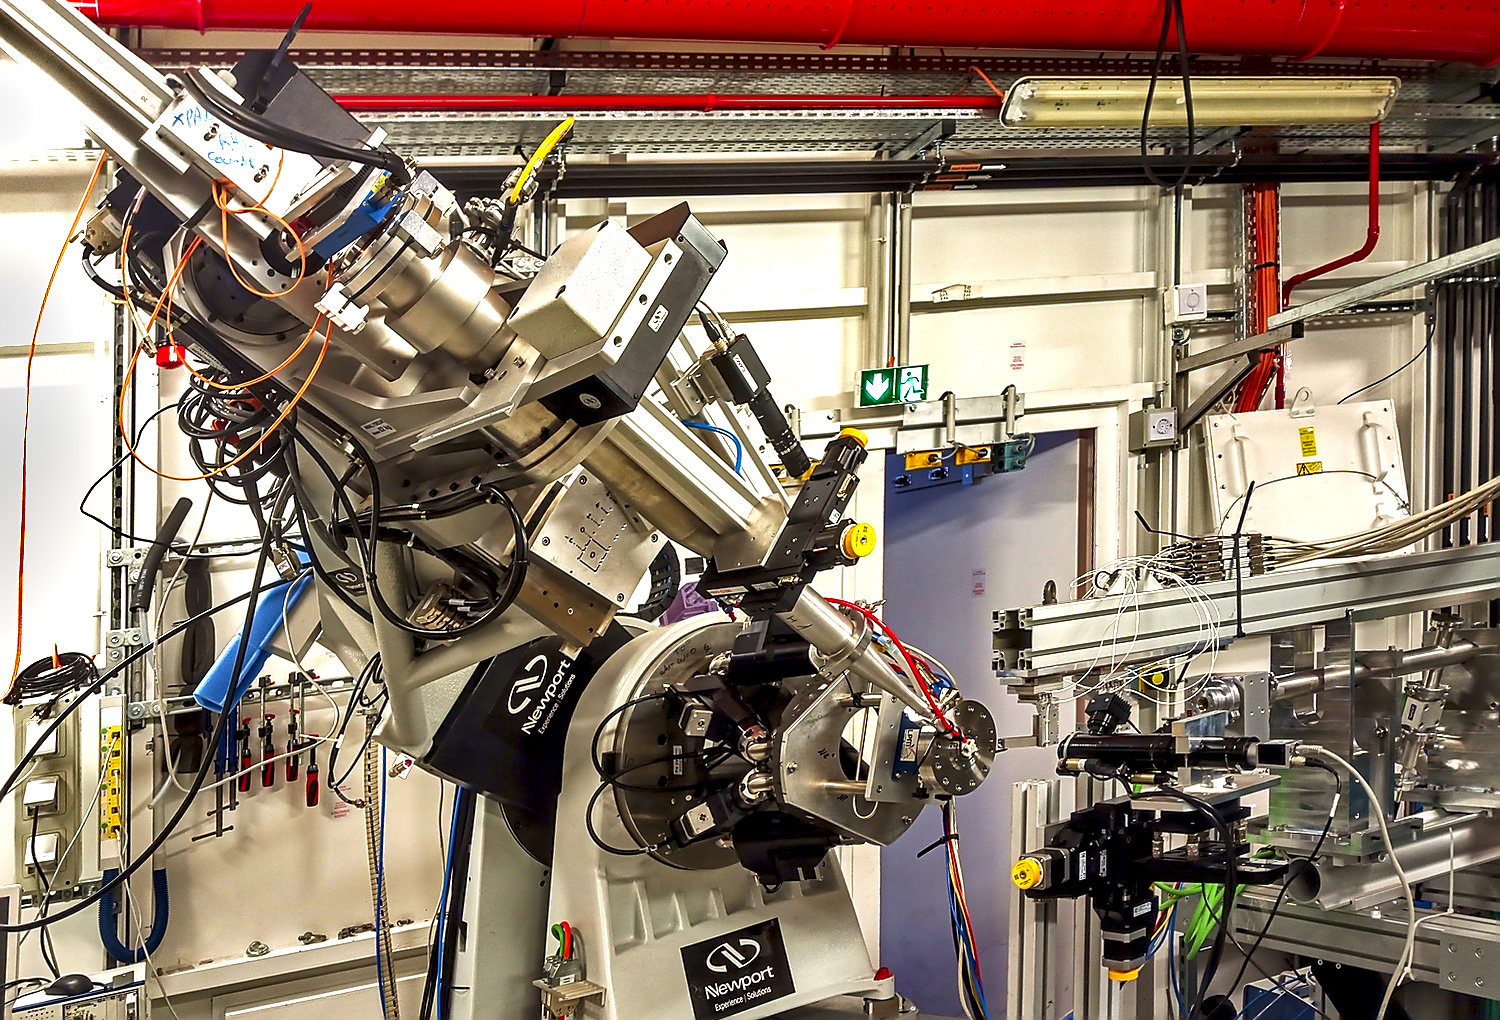
\includegraphics[width=\textwidth]{Figures/sixs/MED.jpg}
        \end{figure}

        \vspace{0.5cm}
        \textit{We would like to thank all the SOLEIL, ESRF and CEA staff for the support and the ERC Carine that supported the research.}

    \end{columns}
\end{frame}
